\newpage
\section{Kết quả và Đánh giá}

\subsection{Kết quả sản phẩm}

\begin{figure}[H]
    \centering
    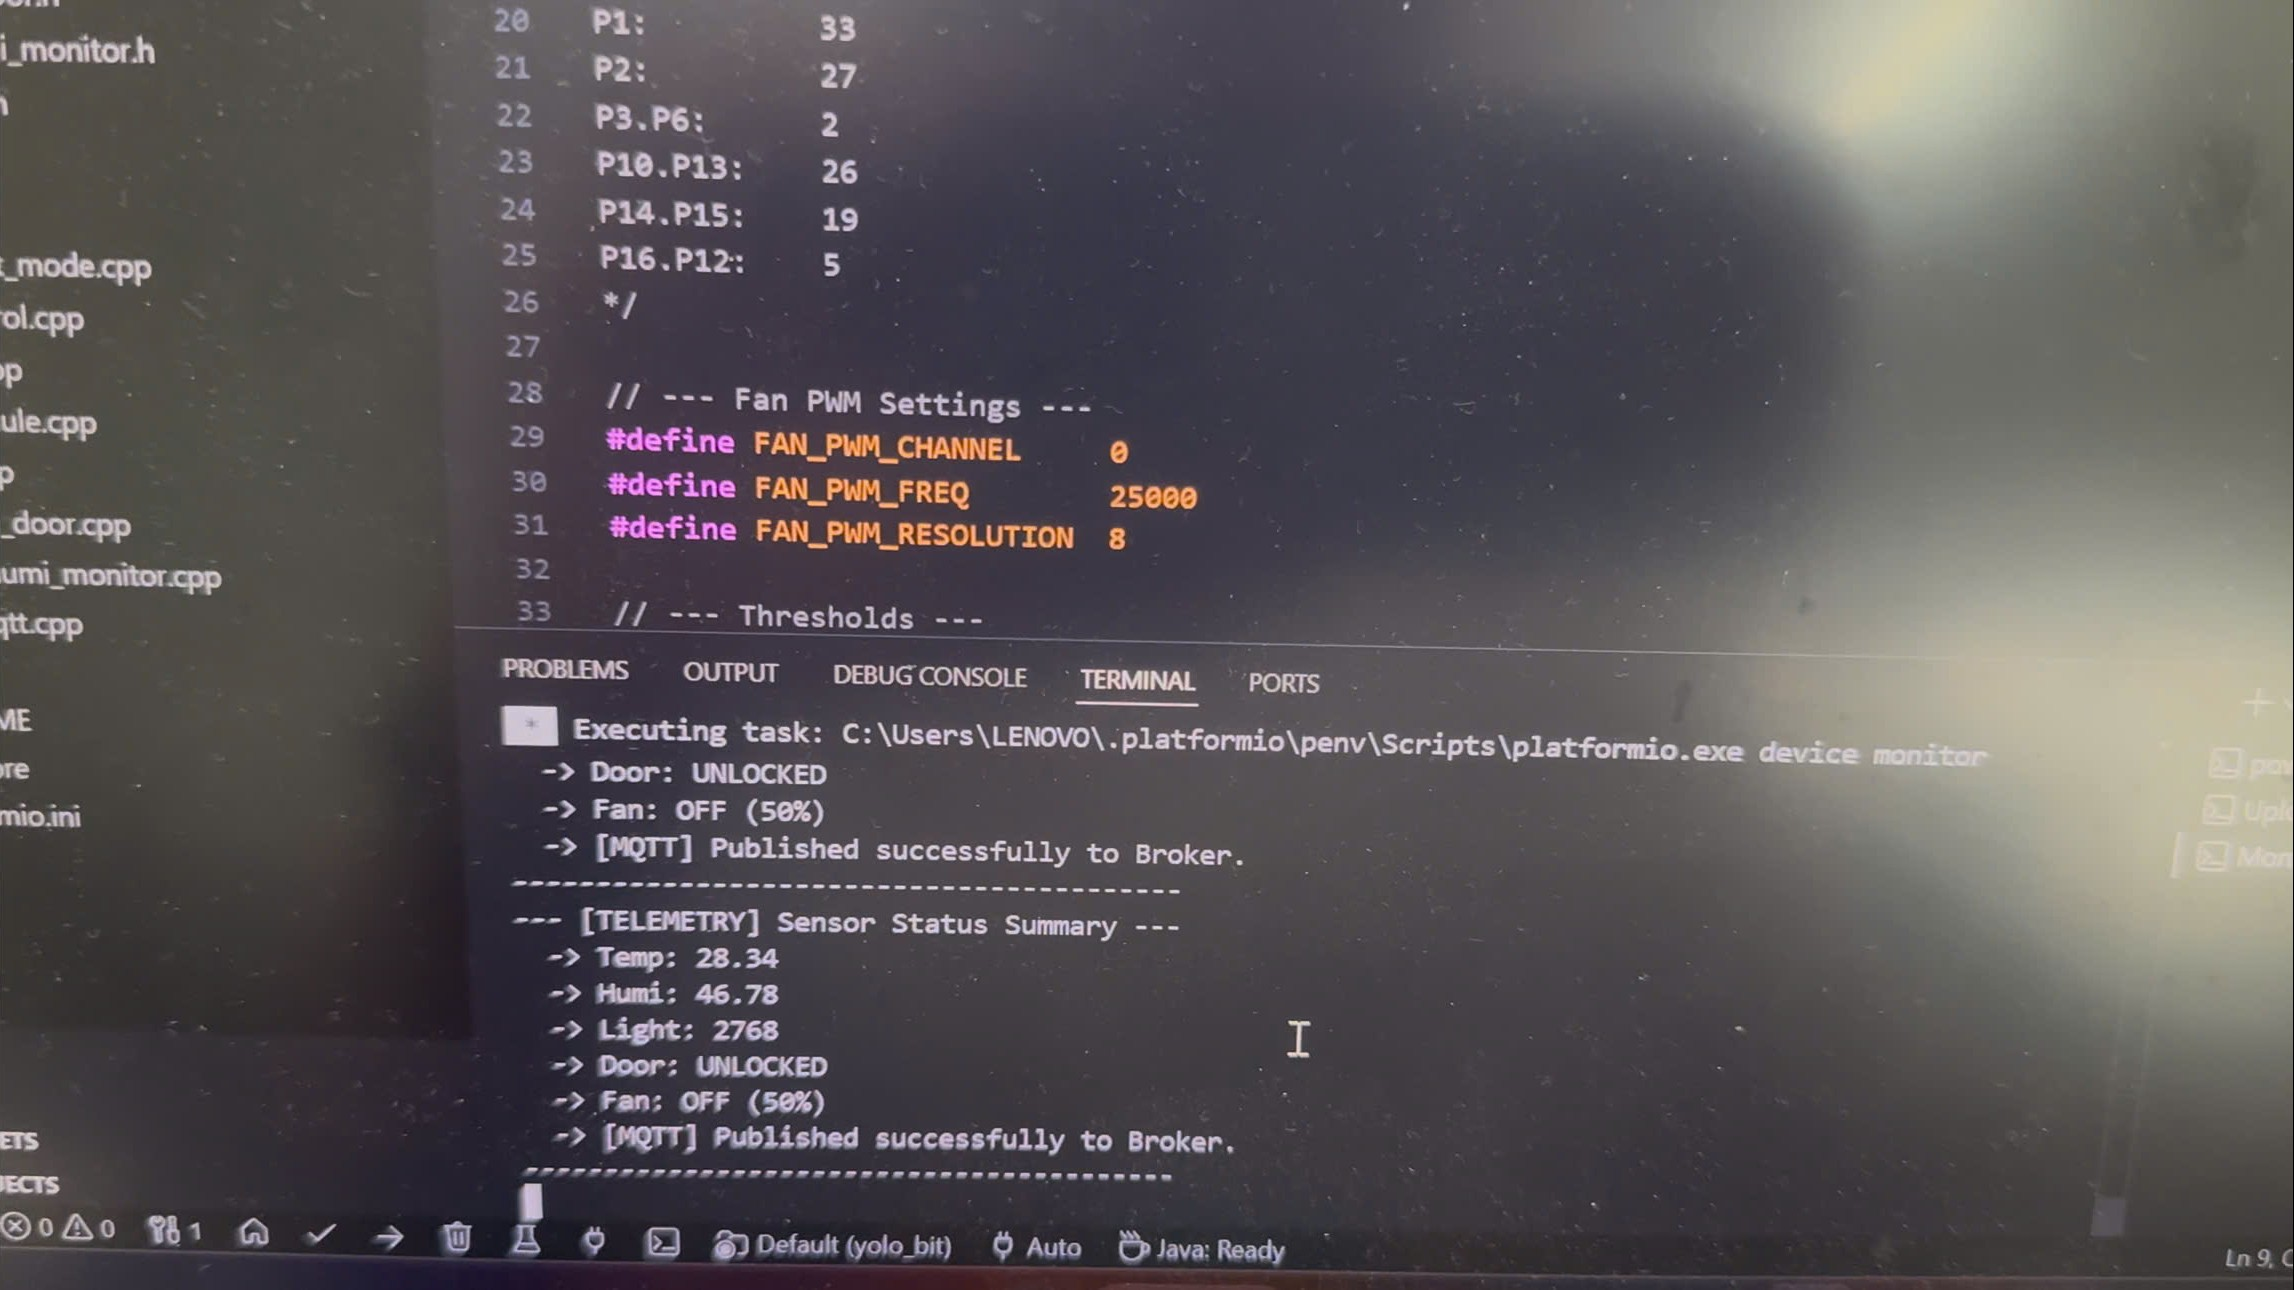
\includegraphics[width=\textwidth]{images/res/monitor.jpg} 
    \caption{Serial Monitor}
    \label{fig:monitor}
\end{figure}

\begin{figure}[H]
    \centering
    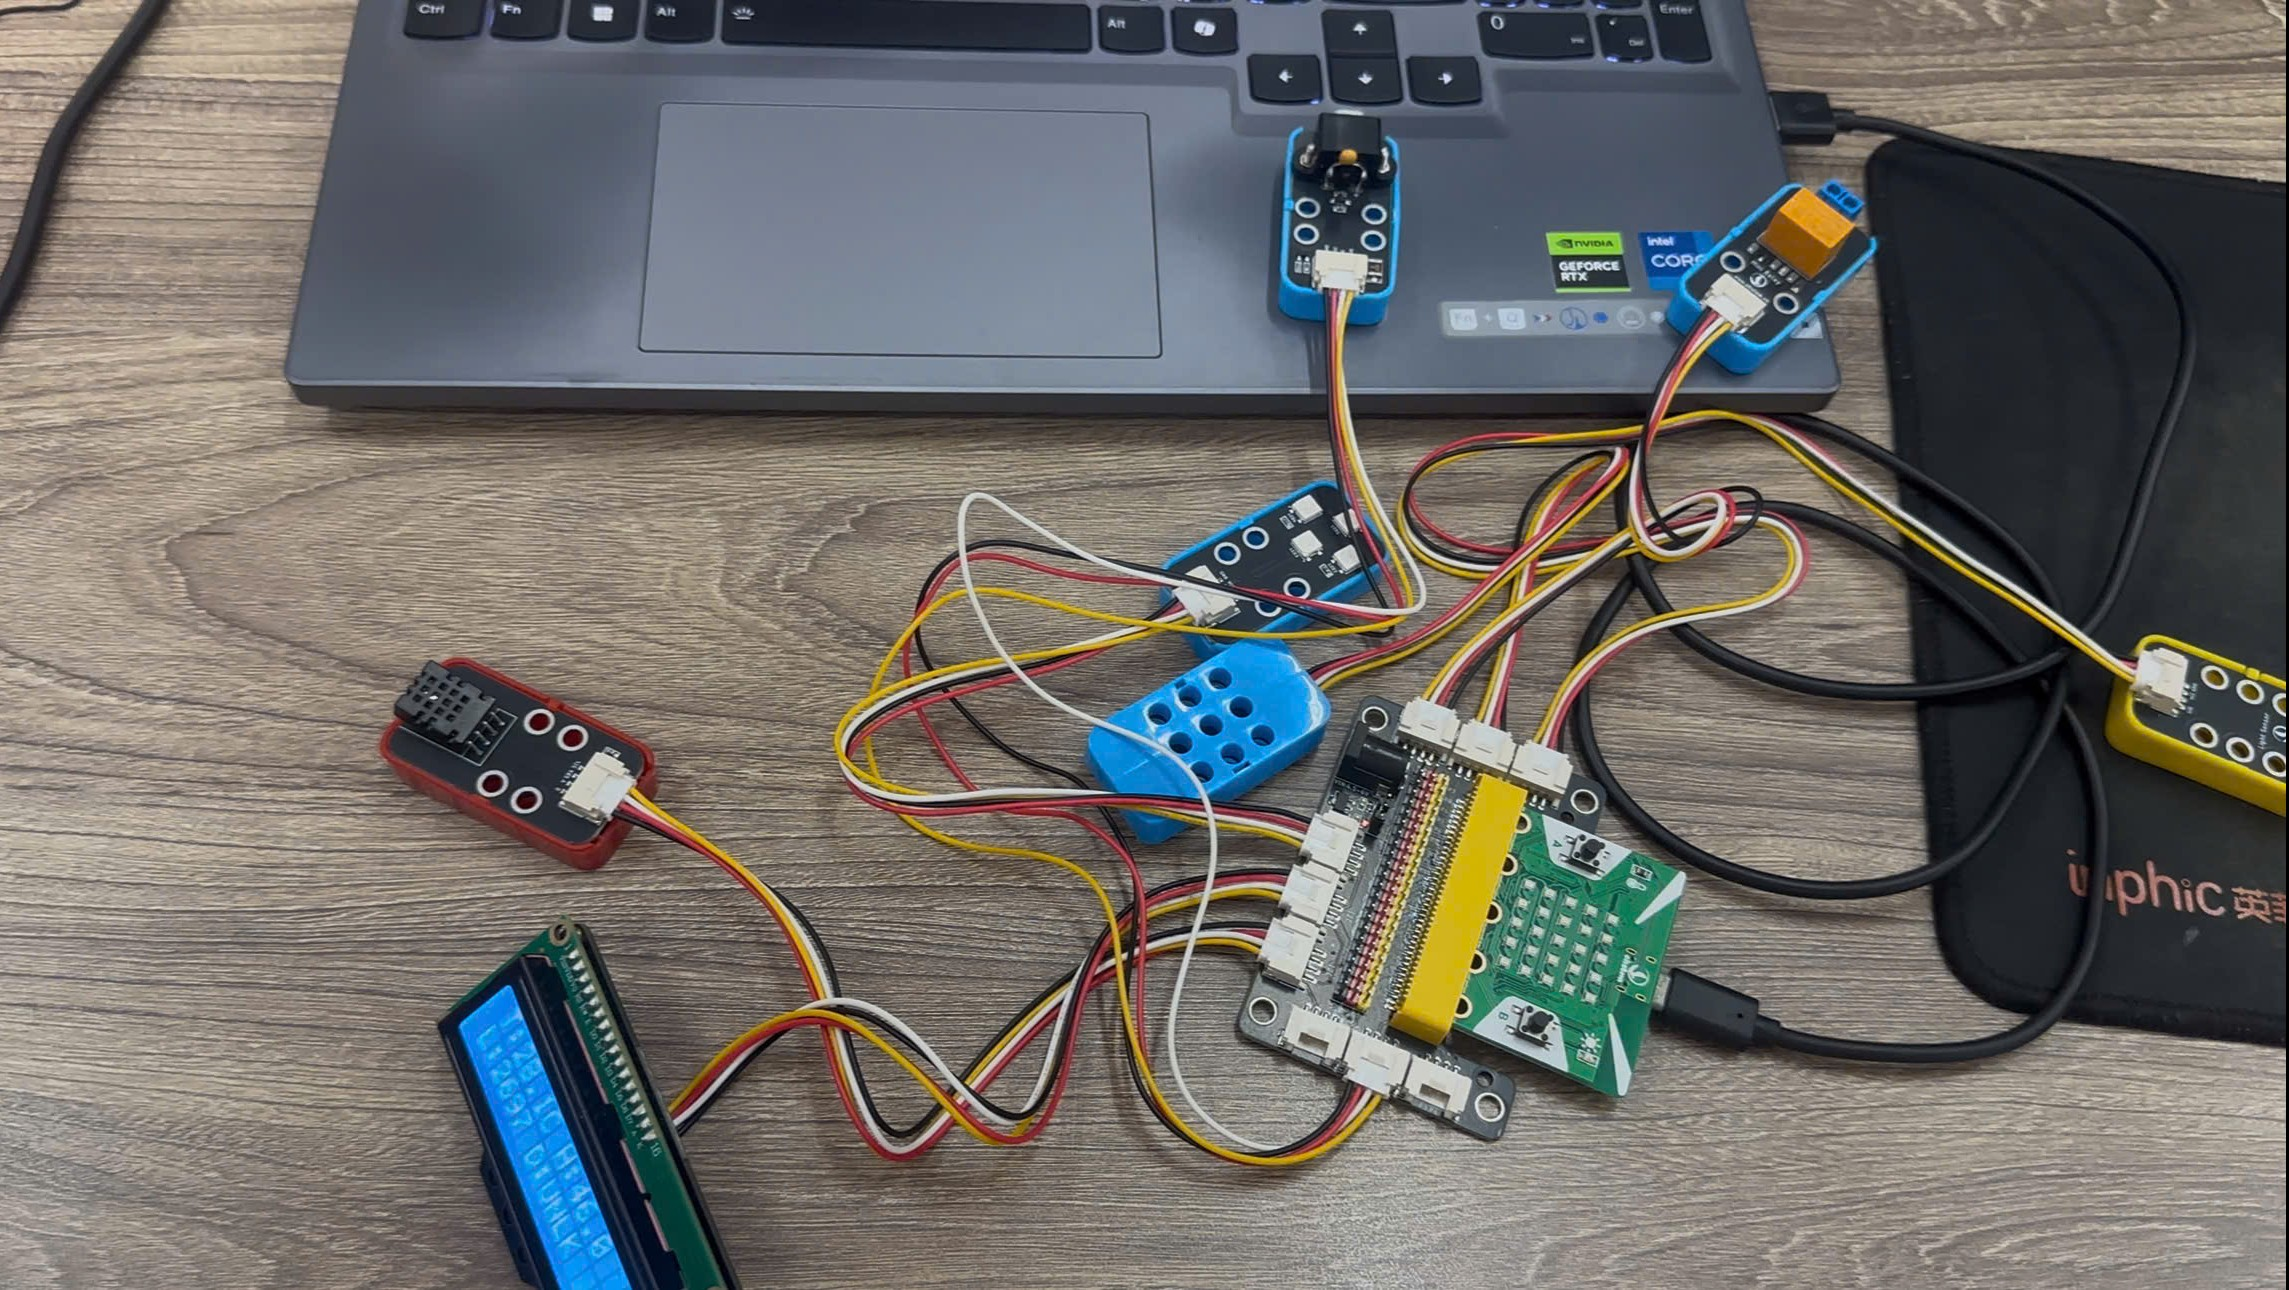
\includegraphics[width=\textwidth]{images/res/hardwares.jpg} 
    \caption{Kết nối mạch}
    \label{fig:hw}
\end{figure}

\begin{figure}[H]
    \centering
    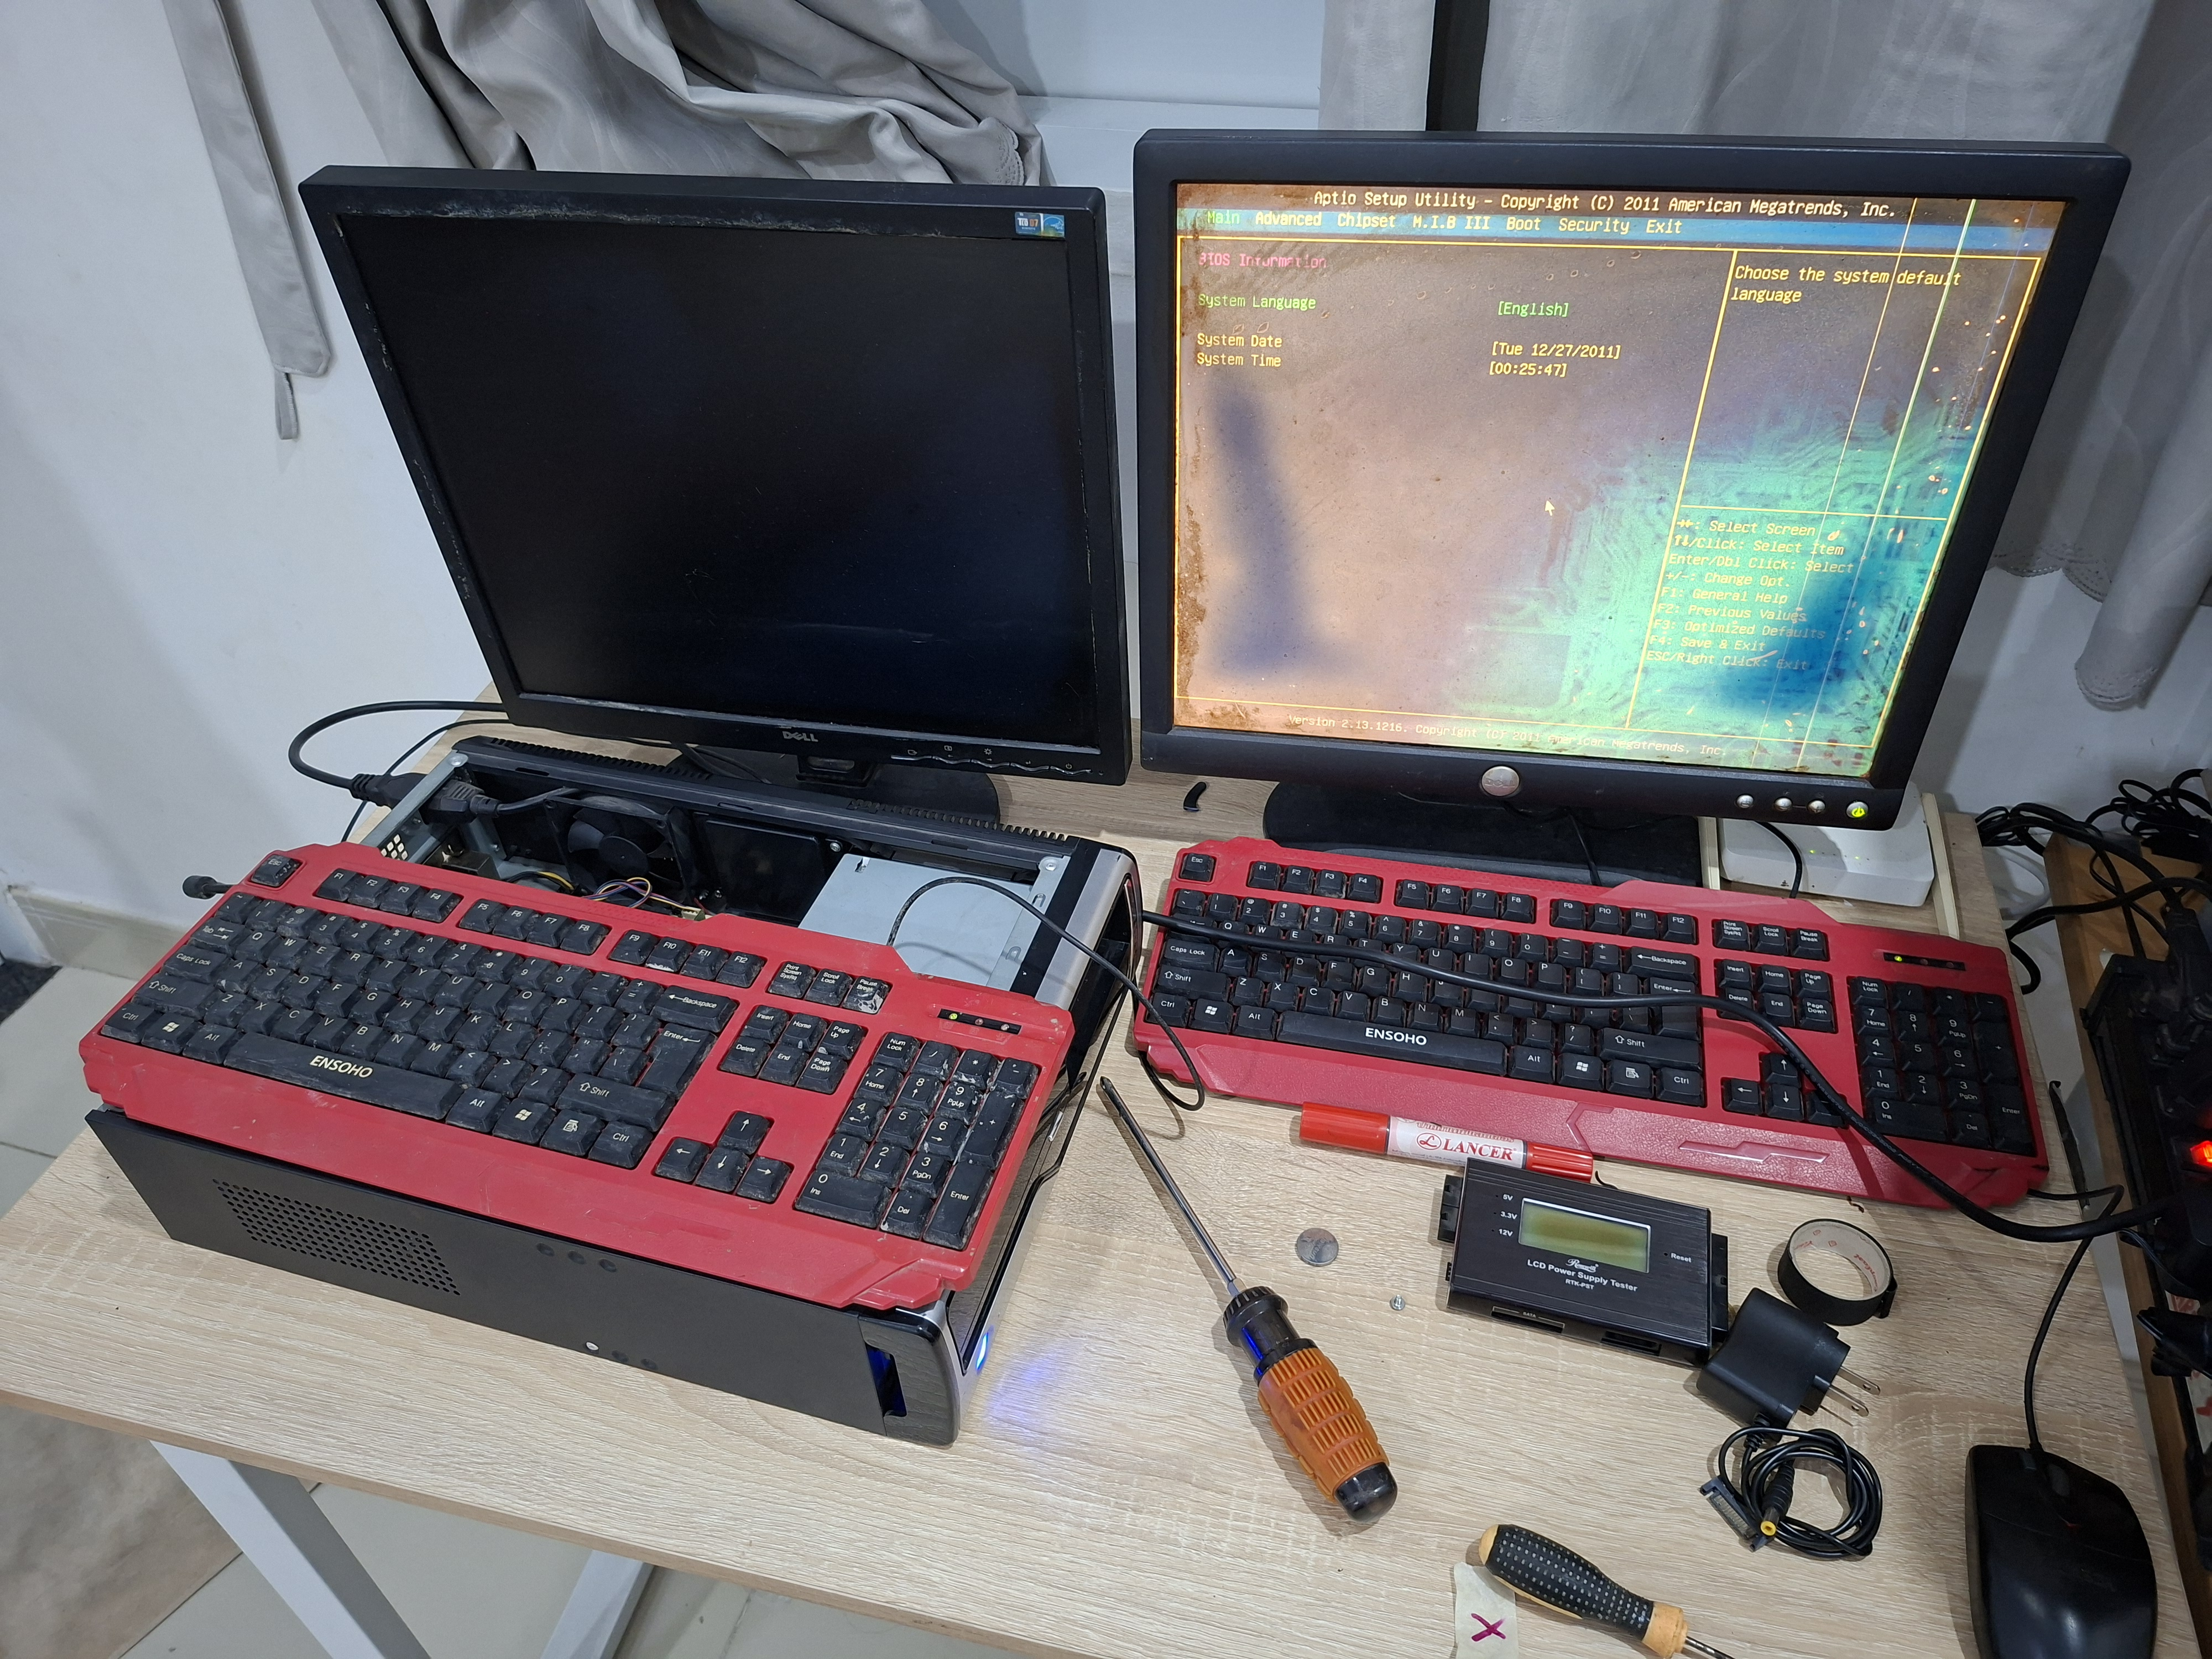
\includegraphics[width=\textwidth]{images/res/server.jpg} 
    \caption{Sửa các phần cứng cũ để tận dùng làm server tại gia}
    \label{fig:sv}
\end{figure}

\begin{figure}[H]
    \centering
    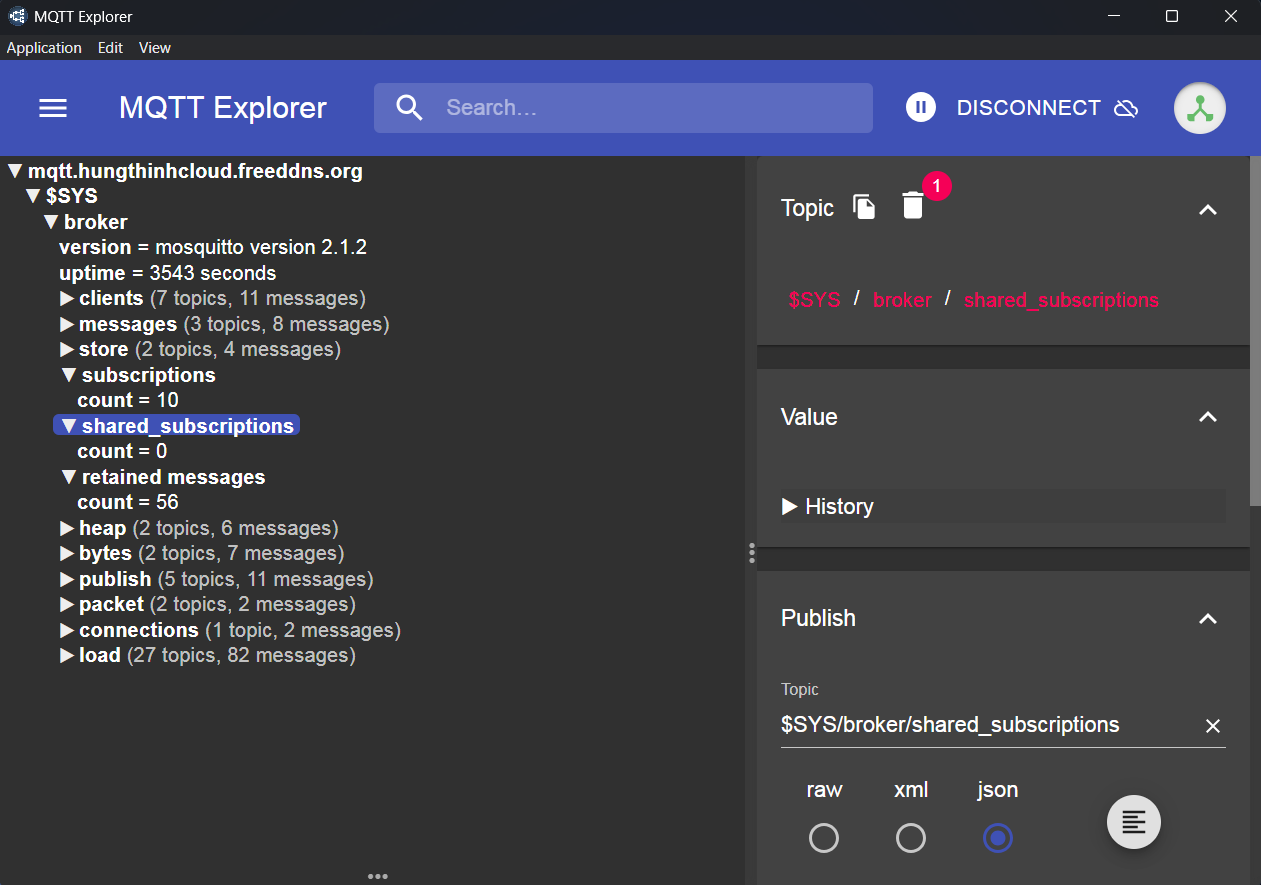
\includegraphics[width=\textwidth]{images/res/mqtt_explorer.png} 
    \caption{MQTT Explorer để quan sát các topic và payload được gửi lên từ thiết bị
Yolo:Bit (Hiện không có topic nào)}
    \label{fig:mqtt}
\end{figure}

\begin{figure}[H]
    \centering
    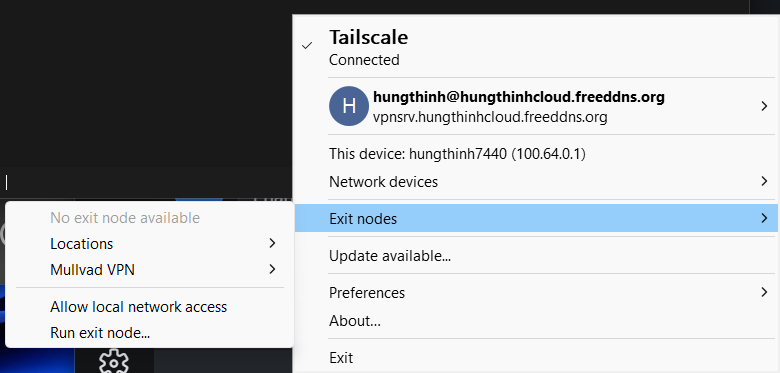
\includegraphics[width=\textwidth]{images/res/vpn.png} 
    \caption{Dev Client kết nối với server thông qua Tailscale VPN}
    \label{fig:vpn}
\end{figure}

\begin{figure}[H]
    \centering
    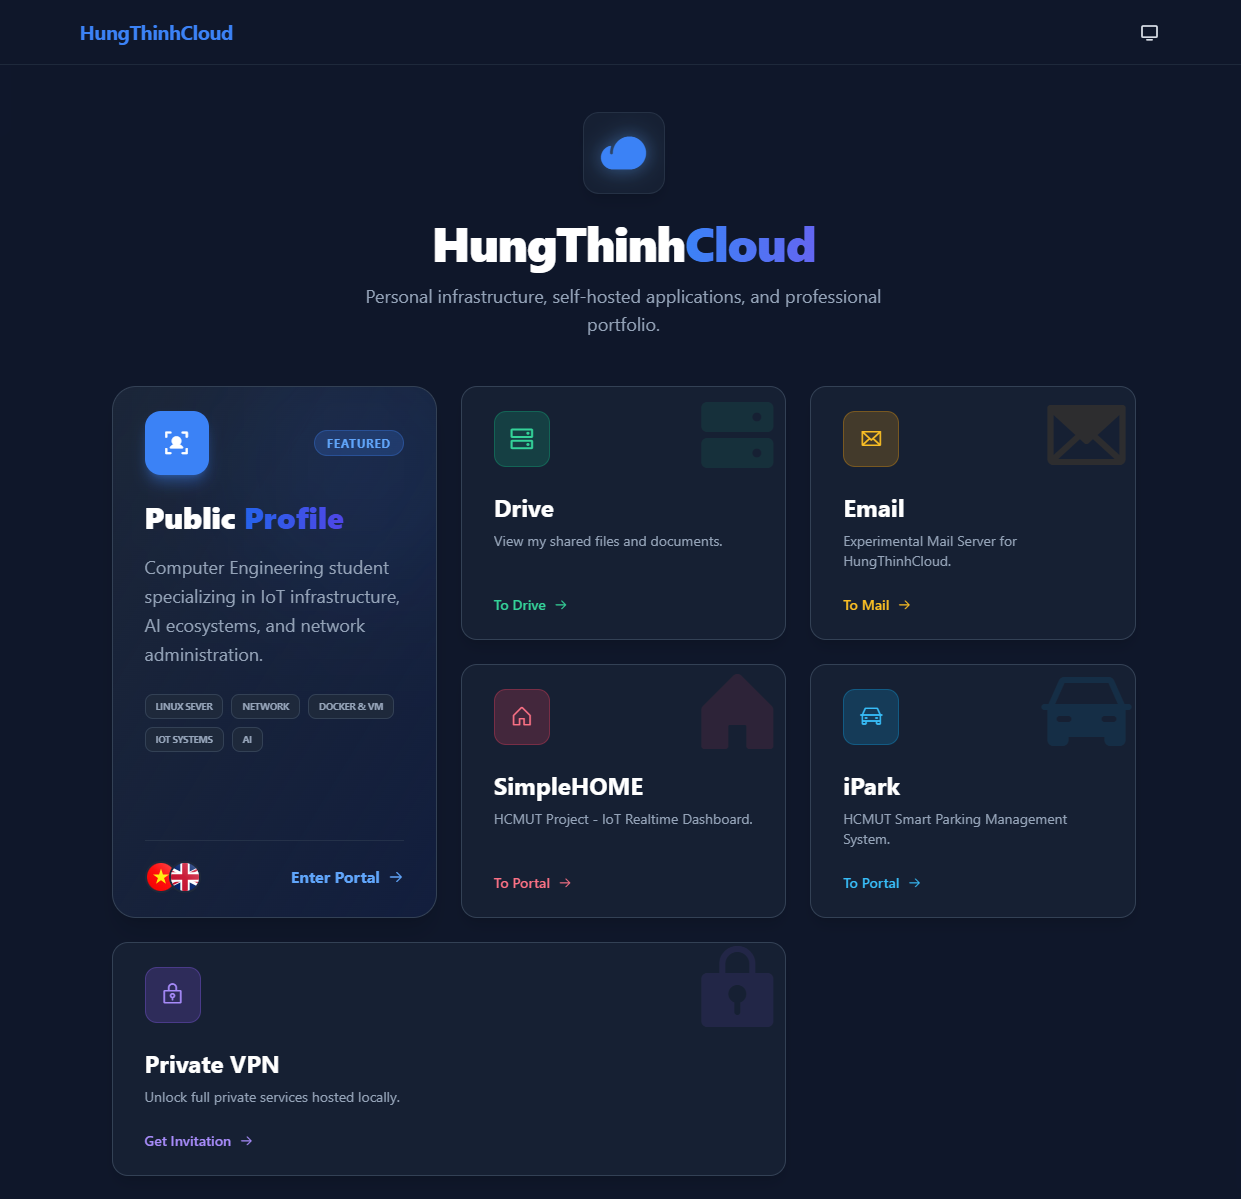
\includegraphics[width=\textwidth]{images/res/homepage.png} 
    \caption{Trang chủ của server HungThinhCloud \url{hungthinhcloud.freeddns.org}}
    \label{fig:db_dark}
\end{figure}

\begin{figure}[H]
    \centering
    
\includegraphics[width=\textwidth]{images/res/homepage_light.png} 
    \caption{Có thể toggle theme sáng, tối, system}
    \label{fig:db_light}
\end{figure}

\begin{figure}[H]
    \centering
    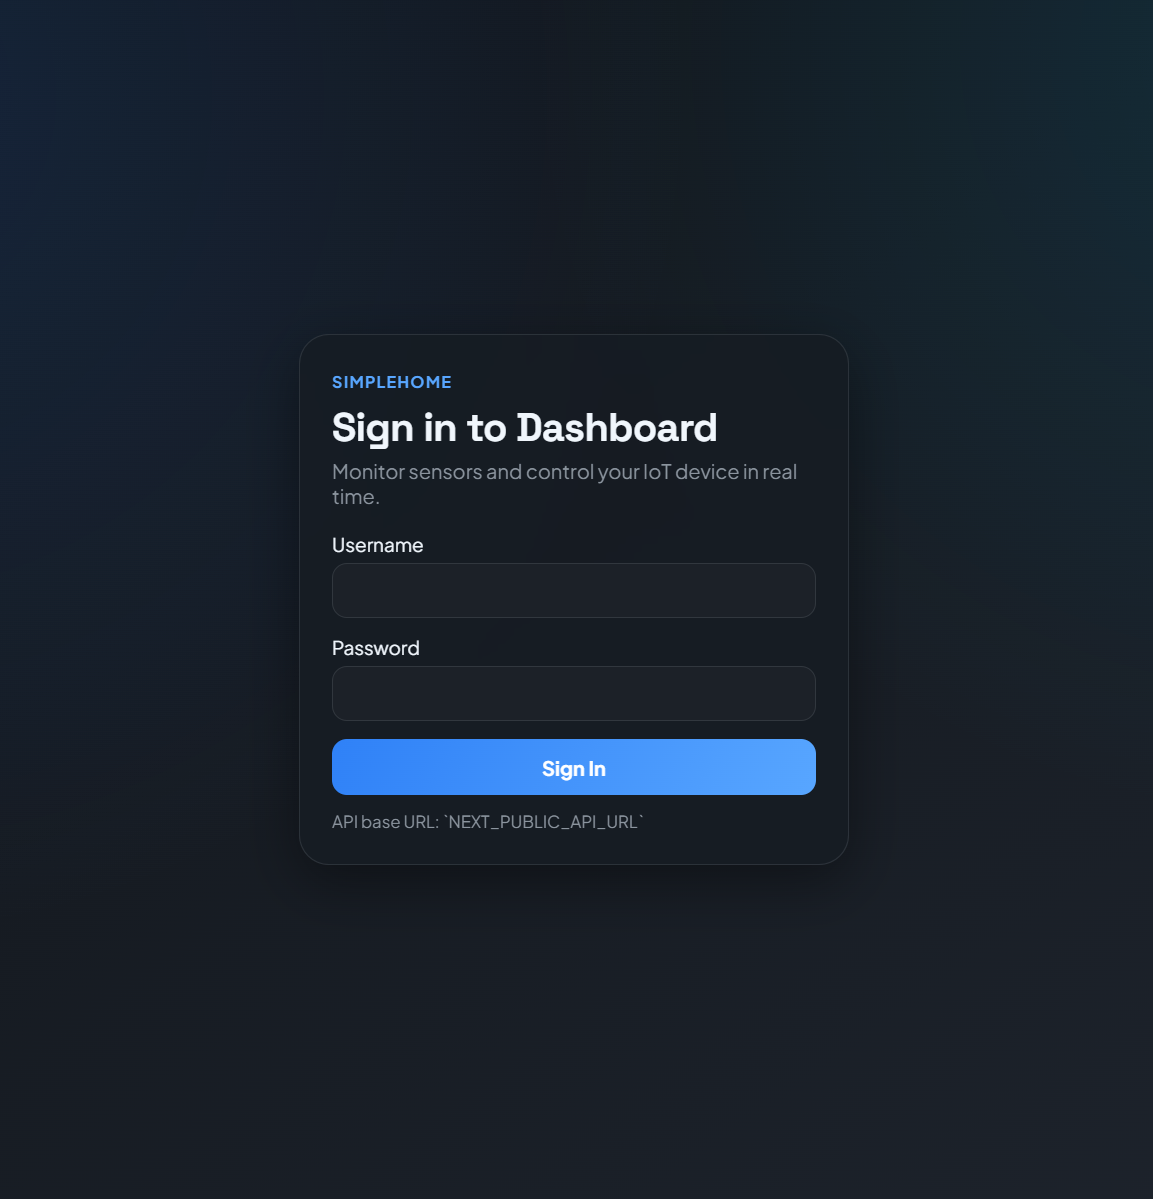
\includegraphics[width=\textwidth]{images/res/login.png} 
    \caption{Giao diện đăng nhập với chủ để theo theme của client}
    \label{fig:login}
\end{figure}

Sau khi nhấn vào card ”SimpleHOME” và đăng nhập thành công, chúng ta sẽ đến với trang dashboard quan sát và điều khiển các thiết bị phần cứng.

\begin{figure}[H]
    \centering
    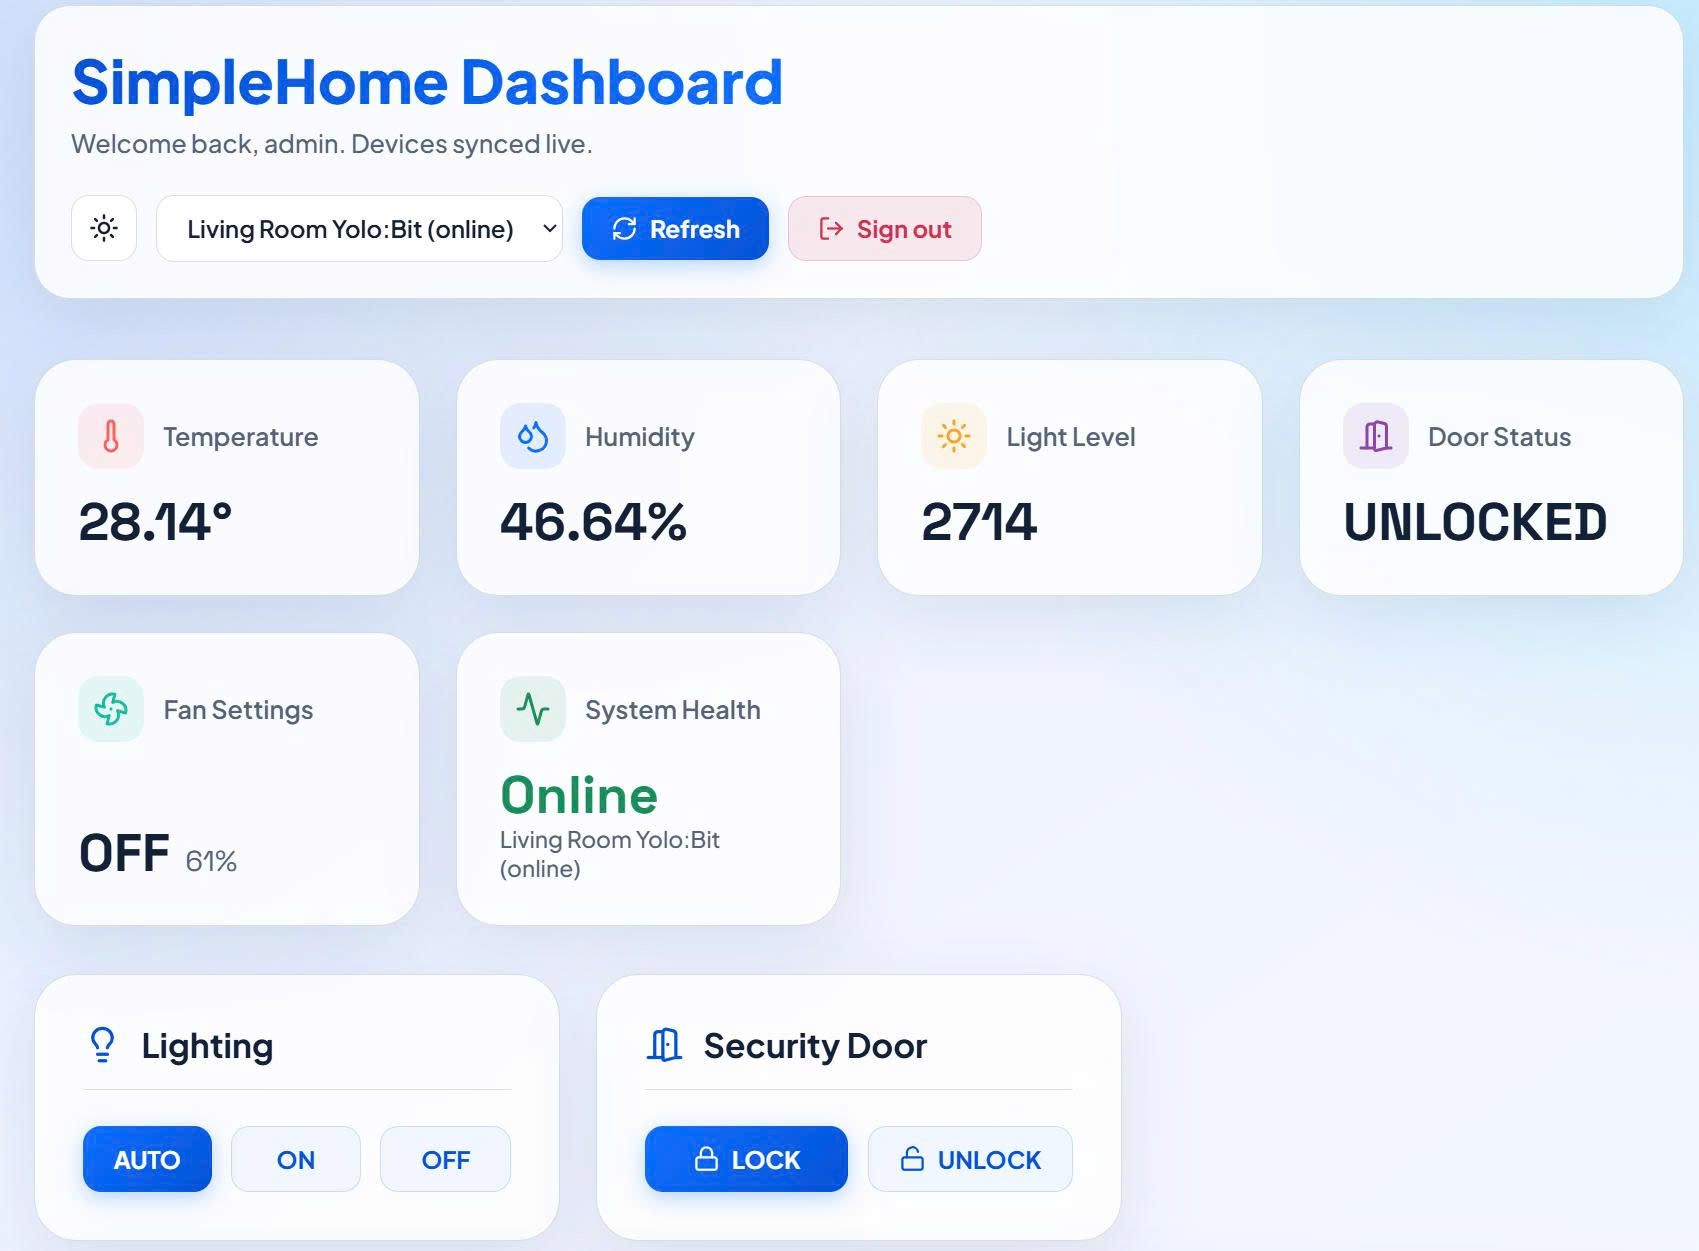
\includegraphics[width=\textwidth]{images/res/db.jpg} 
    \caption{SimpleHome Dashboard}
    \label{fig:db}
\end{figure}

\begin{figure}[H]
    \centering
    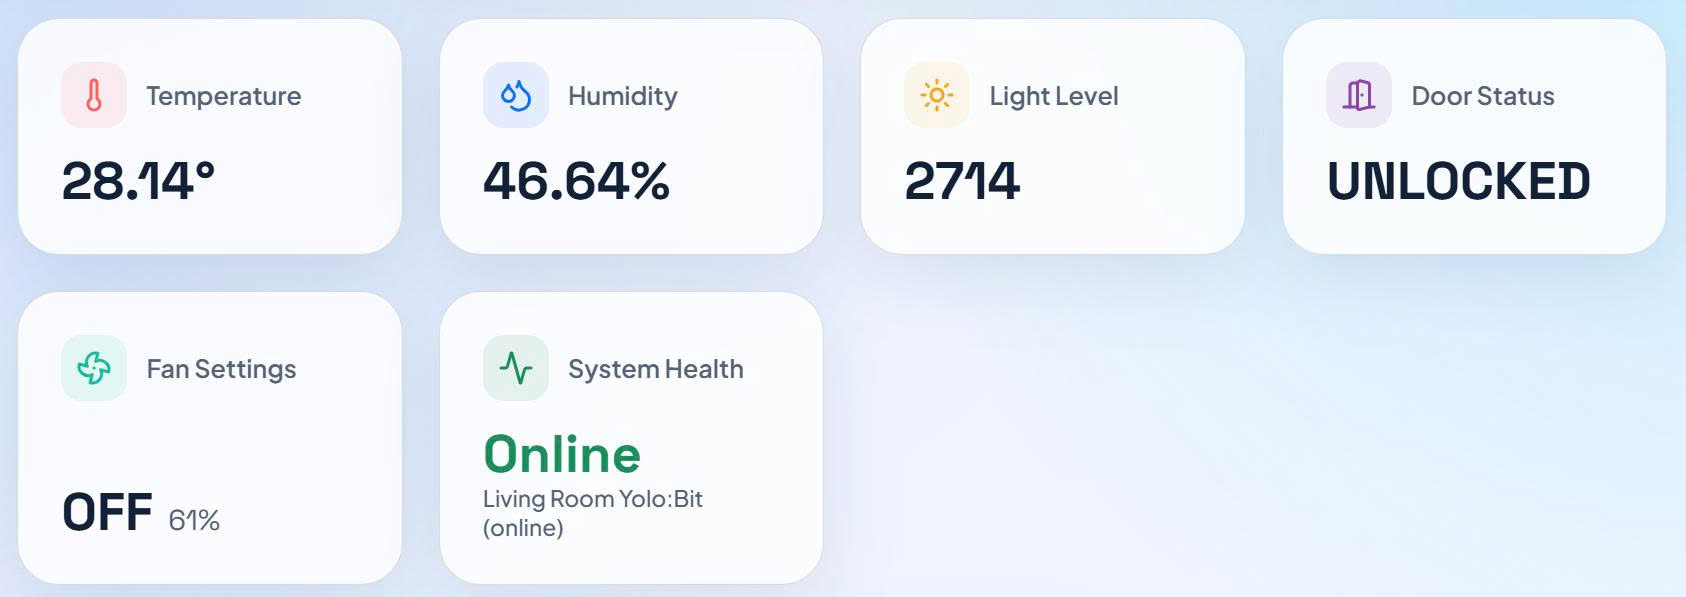
\includegraphics[width=\textwidth]{images/res/monitor_card.jpg} 
    \caption{Các Card để Quan sát dữ liệu của mạch Yolo:Bit}
    \label{fig:monitor_card}
\end{figure}

\begin{figure}[H]
    \centering
    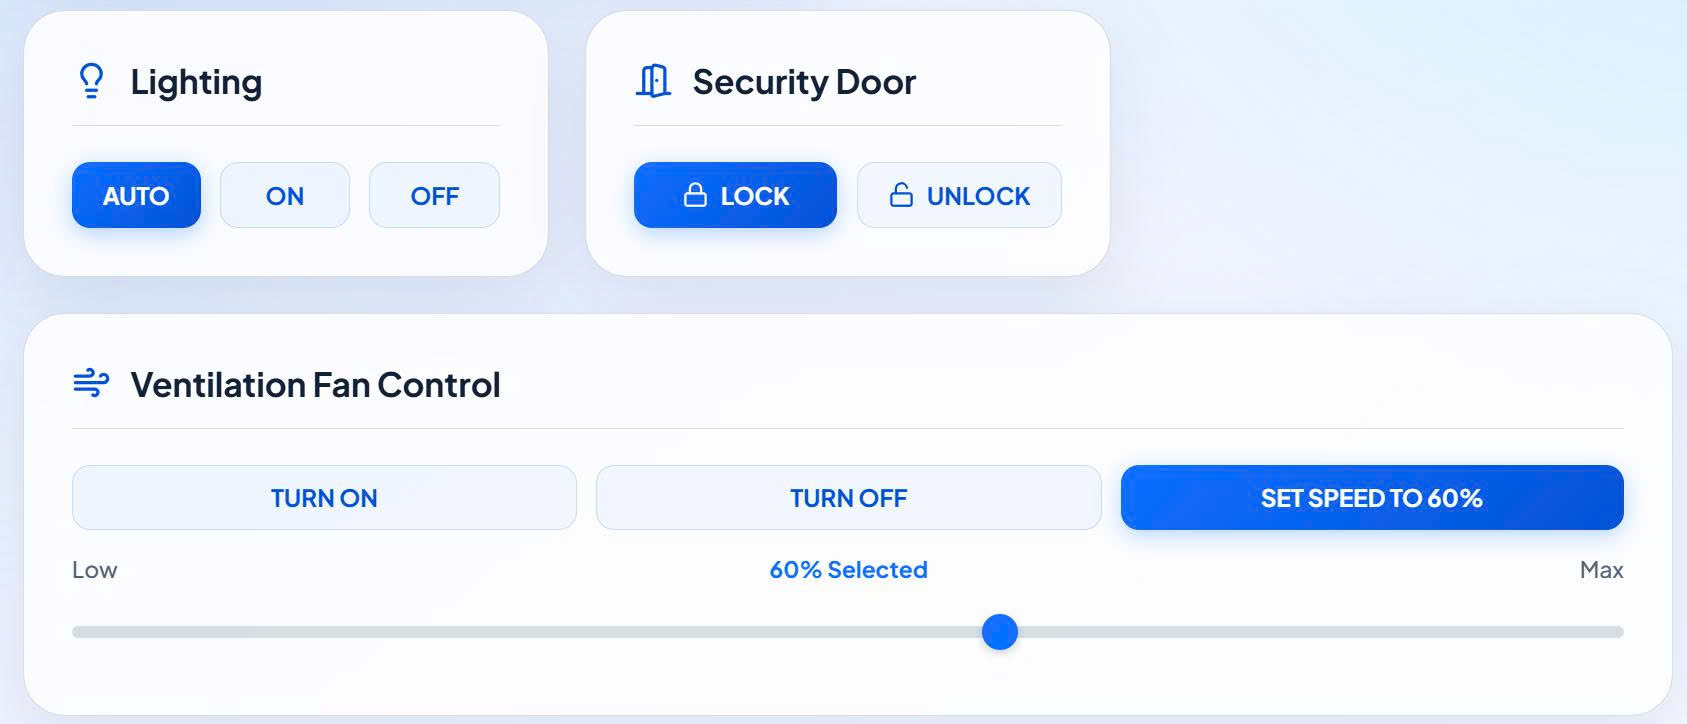
\includegraphics[width=\textwidth]{images/res/control_card.jpg} 
    \caption{Các Card để Điều khiển phần cứng được cắm vào mạch}
    \label{fig:control_card}
\end{figure}

Đây là một trang dashboard IoT tiêu chuẩn cho một hệ thống Nhà thông minh như Yolo Home. Chúng có các Card dùng để quan sát các dữ liệu như:
\begin{itemize}
    \item Nhiệt độ, Độ ẩm được lấy từ DHT20.
    \item Cường độ ánh sáng được đo từ Cảm biến ánh sáng.
    \item Trạng thái cửa đóng/mở.
    \item Trạng thái bật/tắt và tốc độ của quạt
    \item Và cuối cùng là trạng thái của toàn bộ hệ thống.
\end{itemize}
Ngoài ra còn có các Card điều khiển:
\begin{itemize}
    \item Card Lighting với 3 mode AUTO, ON, OFF
    \begin{itemize}
        \item Mode AUTO: Đèn sẽ tự động bật/tắt tùy theo giá trị cường độ ánh sáng được đo từ cảm biến ánh sáng. Nếu trời ”tối” thì tự động bật đèn, nếu trời ”sáng” thì tự động tắt đèn.
        \item MODE ON: Bật đèn ngay lập tức, đèn sẽ được bật cho đến khi chuyển qua các mode khác.
        \item MODE OFF: Tắt đèn, hoạt động tương tự như mode ON.
    \end{itemize}
    \item Card Security Door với 2 mode LOCK và UNLOCK
    \begin{itemize}
        \item Mode LOCK: Như tên gọi, cửa sẽ ngay lập tức đóng lại. Ngoài ra khi đóng cửa, nếu cảm biến IR phát hiện chuyển động (có người), hệ thống sẽ phát cảnh báo về serial monitor.
        \item MODE UNLOCK: Mở cửa.
    \end{itemize}
    \item Card Ventilation Fan Control với 3 mode TURN ON, TURN OFF và SET SPEED
    \begin{itemize}
        \item TURN ON: Bật quạt.
        \item TURN OFF: Tắt quạt.
        \item SET SPEED: Điều chỉnh tốc độ quạt, tốc độ quạt có thể quay từ 0 - 100\%.
    \end{itemize}
\end{itemize}

\subsection{Đánh giá chung}
Tài liệu này trình bày kết quả chức năng chính của hệ thống Simplehome dưới dạng mô tả và quan sát thực nghiệm, không kèm số liệu định lượng. Trong quá trình kiểm thử thực tế bằng các board Yolo Bit (ESP32) và môi trường Docker Compose, hệ thống vận hành đạt các tiêu chí sau:
\begin{itemize}
    \item Hoạt động chức năng: Các thiết bị có thể kết nối tới broker MQTT, gửi dữ liệu telemetry và nhận lệnh điều khiển; backend nhận và lưu trữ dữ liệu vào cơ sở dữ liệu; frontend hiển thị dữ liệu thời gian thực và nhận lệnh người dùng.
    \item Tính chính xác về chức năng: Các thao tác điều khiển (ví dụ bật/tắt thiết bị) phản hồi đúng theo mong đợi trong kịch bản thử nghiệm, và hành động người dùng được ghi nhận vào nhật ký điều khiển (audit logs).
    \item Trải nghiệm người dùng: Giao diện dashboard hiển thị rõ ràng trạng thái thiết bị, cho phép điều hướng giữa các biểu đồ lịch sử và bảng điều khiển, đồng thời hỗ trợ thay đổi theme như minh họa trong hình trước.
    \item Tính bền vững cơ bản: Trong các lần thử cắm/mở lại thiết bị và khởi động lại container, hệ thống vẫn khôi phục kết nối và tiếp tục ghi nhận dữ liệu (behavior cơ bản đã được kiểm chứng bằng thao tác thủ công).
\end{itemize}

\subsection{Hạn chế và quan sát}
Mặc dù hệ thống vận hành đúng chức năng, một số hạn chế quan sát được mà không cần đo lường chính thức bao gồm:
\begin{itemize}
    \item Việc truyền qua mạng Wi‑Fi có thể gây mất gói hoặc trễ tạm thời trong điều kiện tín hiệu yếu; cơ chế retry ở tầng MQTT cần được tinh chỉnh khi triển khai thực tế.
    \item Một số cảnh báo về xử lý file (ví dụ xử lý ảnh SVG nếu không có Inkscape) xuất hiện trong quá trình biên dịch tài liệu; đây là vấn đề của môi trường build, không ảnh hưởng tới logic hệ thống.
    \item Các kiểm thử hiện tại chủ yếu là thủ công và cục bộ; để đánh giá chính xác hiệu năng và khả năng mở rộng cần bổ sung kịch bản tải (load test) và thu thập số liệu.
\end{itemize}

\subsection{Kết luận đánh giá}
Tóm lại, hệ thống đã hoàn thành các chức năng chính theo mục tiêu đồ án ở mức thực nghiệm: kết nối thiết bị, truyền dữ liệu, lưu trữ và hiển thị. Các bước tiếp theo nên tập trung vào đo lường định lượng, tự động hóa kiểm thử và gia cố bảo mật trước khi tiến hành triển khai quy mô lớn.